% biblatex-mla.tex v1.9 2016/11/01
% Maintained at <https://github.com/jmclawson/biblatex-mla/> by James Clawson.
%
% This material is subject to the LaTeX Project Public License. Feel free to improve, redistribute, and adapt to your own ends, as allowed by that license. (See http://www.ctan.org/tex-archive/help/Catalogue/licenses.lppl.html for license details.) For inclusion in future versions, please share improvements in formatting and MLA standards compliance back to James Clawson: <biblatex-mla@konx.net>.
%
% File is in constant progress. Things are messy. Ignore platypi.

\documentclass{ltxdockit}[2011/03/25]
\usepackage{xcolor}
\usepackage{btxdockit}
\usepackage[latin9]{inputenc}
\usepackage[american]{babel}
\usepackage[strict]{csquotes}
\usepackage[style=mla,mancitepar=false]{biblatex}
\usepackage{tabularx}
\usepackage{booktabs}
\usepackage{shortvrb}
\usepackage{libertine}
\usepackage[scaled=0.8]{beramono}
\usepackage{microtype}
\usepackage{graphicx}
\usepackage{hyperref}
\hypersetup{colorlinks,% 
citecolor=black,% 
% filecolor=black,% 
% linkcolor=black,% 
% urlcolor=black}
}

\addbibresource{handbooksamples.bib}

\MakeAutoQuote{<}{>}
\MakeShortVerb{\|}

\newcommand*{\biblatexmla}{\sty{biblatex-mla}\xspace}
\newcommand*{\Biblatexmla}{\sty{Biblatex-mla}\xspace}
\newcommand*{\biblatexcms}{\sty{biblatex-chicago}\xspace}
\newcommand*{\biblatexmlahome}{https://github.com/jmclawson/biblatex-mla/}
\newcommand*{\biblatexmlaonctan}{http://www.ctan.org/tex-archive/help/Catalogue/entries/biblatex-mla.html}
\newcommand*{\mycode}[1]{\texttt{\textbf{#1}}}% things the user needs to type
% Use \sty{} to indicate technical things the user will never type.
\newcommand*{\mylink}[1]{$<$\url{#1}$>$}
\newcommand*{\mla}{MLA\xspace}
\newcommand*{\mycommand}[1]{\mycode{\textbackslash{}#1}}
\newcommand{\superscript}[1]{\ensuremath{^{\textrm{\tiny{#1}}}}}

\newcommand*{\biber}{\sty{biber}\xspace}
\newcommand*{\biblatex}{\sty{Biblatex}\xspace}
\newcommand*{\biblatexhome}{http://sourceforge.net/projects/biblatex/}
\newcommand*{\biblatexctan}{http://www.ctan.org/tex-archive/macros/latex/contrib/biblatex/}

\makeatletter
\def\subsubsection{\@startsection{subsubsection}{3}{-2.2em}{-5.25ex plus -1ex minus -.2ex}{0.5ex plus .2ex}{\large\textbf}}
\newenvironment*{commandlist}
  {\list{}{%
     \setlength{\labelwidth}{\marglistwidth}%
     \setlength{\labelsep}{\marglistsep}%
     \setlength{\leftmargin}{0pt}%
     \renewcommand*{\makelabel}[1]{\hss\marglistfont##1}}%
   \def\commanditem##1{%
     \item[{\textbackslash{}##1}]%
     \ltd@pdfbookmark{##1}{##1}}}
  {\endlist}
\newenvironment*{optionslist}
  {\list{}{%
     \setlength{\labelwidth}{\marglistwidth}%
     \setlength{\labelsep}{\marglistsep}%
     \setlength{\leftmargin}{0pt}%
     \renewcommand*{\makelabel}[1]{\hss\marglistfont##1}}%
   \def\optionitem##1{%
     \item[{##1}]%
     \ltd@pdfbookmark{##1}{##1}}}
  {\endlist}
\newenvironment*{optionslistNOT}
  {\list{}{%
     \setlength{\labelwidth}{\marglistwidth}%
     \setlength{\labelsep}{\marglistsep}%
     \setlength{\leftmargin}{50pt}%
     \renewcommand*{\makelabel}[1]{\hss\marglistfont##1}}%
   \def\optionitem##1{%
     \item[{\textbf{##1}}]}}
  {\endlist}
\makeatother


\titlepage{%
  title={\biblatexmla},
  subtitle={\mla{} Style Using \biblatex},
  url={\biblatexmlahome},
  author={James Clawson},
  email={biblatex-mla@konx.net},
  revision={1.9},
  date={\today}}

\hypersetup{%
  pdftitle={biblatex-mla},
  pdfsubject={MLA Style Using biblatex},
  pdfauthor={James Clawson},
  pdfkeywords={mla, biblatex, bibtex, bibliography, citation}}

% colors

\definecolor{spot}{rgb}{1,0.5,0}

% tables

\newcolumntype{V}{>{\raggedright\let\\=\tabularnewline\ttfamily}p}
\newcolumntype{H}{>{\sffamily\bfseries\spotcolor}l}
\newcolumntype{P}{>{\raggedright}p{100pt}}
\newcolumntype{O}{>{\raggedright\ttfamily}p{40pt}}
\newcolumntype{S}{>{\raggedright\ttfamily}X}
\newcolumntype{N}{>{\sffamily\bfseries\spotcolor}r}
\newcolumntype{n}{>{\raggedleft\let\\\tabularnewline}p{50pt}}

\providecommand*{\numtablesetup}{\tablesetup}

\newcommand*{\sorttablesetup}{%
  \tablesetup
  \setlength{\tabcolsep}{1pt}%
  \def\new{\ensuremath\rightarrow}%
  \def\alt{\ensuremath\hookrightarrow}%
  \def\str##1{\mbox{\displayverbfont##1}}%
  \def\altstr##1{\hfill\alt\hspace{2\tabcolsep}%
    \str{##1}\hspace*{2\tabcolsep}}%
  \let\fld\bibfield}

% markup and misc

\setcounter{secnumdepth}{4}

\newrobustcmd*{\BiberOnly}{%
  \textcolor{spot}{Biber only}}
\newrobustcmd*{\BiberOnlyMark}{%
  \leavevmode\marginpar{\BiberOnly}}

\hyphenation{%
  star-red
  bib-lio-gra-phy
  white-space
  bib-latex
}

\newcommand*{\mlabibbox}[2]{\begin{center}\colorbox{#1!30}{\parbox{.9\linewidth}{#2}}\end{center}}
\newcommand*{\mlaprintbox}[2]{\begin{center}\colorbox{#1!30}{\parbox{.9\linewidth}{\begin{center}\textbf{Works Cited}\end{center}#2}}\end{center}}

\DeclareFieldFormat{braces}{\{#1\}}%
\DeclareNameAlias{default}{first-last}%
\DeclareNameAlias{author}{first-last}%
\DeclareNameAlias{editor}{first-last}%
\DeclareNameAlias{translator}{first-last}%
\DeclareNameAlias{namea}{first-last}%
\DeclareNameAlias{nameb}{first-last}%
\DeclareNameAlias{namec}{first-last}%
\DeclareListFormat{location}{%
  #1%
  \ifthenelse{\value{listcount}<\value{liststop}}
    {\addcomma\space}
    {}}%
\DeclareListFormat[article]{location}{%
  #1%
  \ifthenelse{\value{listcount}<\value{liststop}}
    {\addcomma\space}
    {}}%
\DefineBibliographyExtras{british}{%
  \protected\def\bibdatedash{$/$}
  \def\finalandcomma{}%
  \protected\def\mkbibdatelong#1#2#3{%
    \iffieldundef{#1}
      {}
      {\thefield{#1}\iffieldundef{#2}{}{-}}%
    \iffieldundef{#2}
      {}
      {\thefield{#2}\iffieldundef{#3}{}{-}}%
    \thefield{#3}}}

\renewcommand*{\multinamedelim}{\addspace\bibstring{and}\space}

\newcommand{\mlafullexample}[2]{\newline%
\mlabibbox{orange}{\begin{description}\item\mlaexample{#1}\end{description}}%
\normalfont{#2}\selectlanguage{american}%
\mlaprintbox{white}{\begin{description}\item\normalfont\fullcite{#1}\end{description}}}

\DeclareCiteCommand{\mlaexample}[\texttt]
  {\selectlanguage{british}\printtext{$@$}\printfield{entrytype}}%
  {\{\printfield{entrykey}\usebibmacro{cite:mlaexample}}%
  {}%
  {\selectlanguage{american}}
\newbibmacro*{cite:mlaexample}{%
  \setunit{\addcomma\printtext{\newline}}
  \usebibmacro{cite:mlaexample:internal}{author}%
  \usebibmacro{cite:mlaexample:internal}{authortype}%
  \usebibmacro{cite:mlaexample:internal}{bookauthor}%
  \usebibmacro{cite:mlaexample:internal}{booktitle}%
  \usebibmacro{cite:mlaexample:internal}{booksubtitle}%
  \usebibmacro{cite:mlaexample:internal}{date}%
  \usebibmacro{cite:mlaexample:internal}{edition}%
  \usebibmacro{cite:mlaexample:internal}{editor}%
  \usebibmacro{cite:mlaexample:internal}{editortype}%
  \usebibmacro{cite:mlaexample:internal}{entrysubtype}%
  \usebibmacro{cite:mlaexample:internal}{eprint}%
  \usebibmacro{cite:mlaexample:internal}{eprinttype}%
  \usebibmacro{cite:mlaexample:internal}{howpublished}%
  \usebibmacro{cite:mlaexample:internal}{institution}%
  \usebibmacro{cite:mlaexample:internal}{introduction}%
  \usebibmacro{cite:mlaexample:internal}{journaltitle}%
  \usebibmacro{cite:mlaexample:internal}{location}%
  \usebibmacro{cite:mlaexample:internal}{maintitle}%
  \usebibmacro{cite:mlaexample:internal}{mainsubtitle}%
  \usebibmacro{cite:mlaexample:internal}{nameaddon}%
  \usebibmacro{cite:mlaexample:internal}{namea}%
  \usebibmacro{cite:mlaexample:internal}{nameatype}%
  \usebibmacro{cite:mlaexample:internal}{nameb}%
  \usebibmacro{cite:mlaexample:internal}{namebtype}%
  \usebibmacro{cite:mlaexample:internal}{namec}%
  \usebibmacro{cite:mlaexample:internal}{namectype}%
  \usebibmacro{cite:mlaexample:internal}{number}%
  \usebibmacro{cite:mlaexample:internal}{options}%
  \usebibmacro{cite:mlaexample:internal}{origdate}%
  \usebibmacro{cite:mlaexample:internal}{pages}%
  \usebibmacro{cite:mlaexample:internal}{publisher}%
  \usebibmacro{cite:mlaexample:internal}{series}%
  \usebibmacro{cite:mlaexample:internal}{subtitle}%
  \usebibmacro{cite:mlaexample:internal}{title}%
  \usebibmacro{cite:mlaexample:internal}{titleaddon}%
  \usebibmacro{cite:mlaexample:internal}{translator}%
  \usebibmacro{cite:mlaexample:internal}{type}%
  \usebibmacro{cite:mlaexample:internal}{url}%
  \usebibmacro{cite:mlaexample:internal}{urldate}%
  \usebibmacro{cite:mlaexample:internal}{version}%
  \usebibmacro{cite:mlaexample:internal}{volume}%
  \setunit{\printtext{}}\printtext{\}\selectlanguage{american}%
  }%
}
\newbibmacro{cite:mlaexample:internal}[1]{%
  \ifthenelse{\equal{#1}{date}}{%
    \iffieldundef{year}{}{%
      \printtext{\indent date}%
   	  \printtext{$=$ \addspace}%
	  \printtext[braces]{\printdate}%
	}%
  }{}%
  \ifthenelse{\equal{#1}{origdate}}{%
    \iffieldundef{origyear}{}{
	  \printtext{\indent origdate}%
	  \printtext{$=$ \addspace}%
	  \printtext[braces]{\printorigdate}%
	}%
  }{}%
  \ifthenelse{\equal{#1}{urldate}}{%
    \iffieldundef{urlyear}{}{
	  \printtext{\indent urldate}%
	  \printtext{$=$ \addspace}%
	  \printtext[braces]{\printurldate}%
	}%
  }{}%
  \iffieldundef{#1}{}{%
    \printtext{\indent#1}%
	\printtext{$=$ \addspace}%
	\printfield[braces]{#1}%
  }%
  \ifnameundef{#1}{}{%
    \printtext{\indent#1}%
	\printtext{$=$ \addspace}%
	\printtext[braces]{\printnames{#1}}%
  }%
  \iflistundef{#1}{}{%
    \printtext{\indent#1}%
	\printtext{$=$ \addspace}%
	\printtext[braces]{\printlist{#1}}%
  }%
  \setunit{\addcomma\printtext{\newline}}}




\begin{document}

\printtitlepage
\tableofcontents


% \subsection{Examples} % (fold)
% \label{ssub:examples}
% \autocite{sendak63aa}

% subsection examples (end)

\section{Version Note}
This beta update is for testing compatibility with the 8\superscript{th} edition of the \emph{MLA Handbook}, published April 2016. This current version supports both the old edition (by using \sty{style=mla} in the preamble) and the newer edition (using \sty{style=mla-new}); an upcoming version of \biblatexmla will deprecate support for the 7\superscript{th} edition in favor of the 8\superscript{th}. See \secref{mla:sec:use} for more on switching between editions.

\section{Introduction}
\label{int}

\Biblatexmla provides support to \biblatex, \bibtex, and \latex for citations and Works Cited lists in the style established by the Modern Language Association (\mla). For commands and options to change package defaults, see \secref{mla:subsec:commands} and \secref{mla:subsec:options}, respectively, below.

\mla style, a common standard for writers in the humanities, is outlined in the \emph{MLA Style Manual}, in its 3\superscript{rd} edition, and the \emph{MLA Handbook for Writers of Research Papers}, now in its 8\superscript{th} edition. \Biblatexmla follows the style outlined in the latter of these. It also follows the logic of the \mla{} when citing similar material repeatedly, trimming unnecessary information from citations where necessary. \Biblatexmla is compatible with \biblatex's support for \sty{hyperref} and \sty{tex4ht}, and the main word in each citation (either the author's name, the title, or the page number) serves as a link to the particular entry in the Works Cited. For anything not covered by this manual, please also see the \biblatex documentation or contact me by email.

\newpage
\section{Use}
\label{mla:sec:use}

To ensure American-style quotation marks (if that's your thing),%
%%
\footnote{Other localization files, \sty{mla-spanish.lbx}, \sty{mla-portuguese.lbx}, and \sty{mla-italian.lbx}, are also available to use \biblatexmla in languages other than English. These and other localization files are included in \biblatexmla releases, but they will not always be the latest versions available. Updated and new localization files will be kept on GitHub (\mylink{\biblatexmlahome}) once they are ready. There is also support for proper punctuation in non-American dialects of English. Try \mycode{british}, \mycode{canadian}, or other Babel identifiers, such as \mycode{spanish}.} %
%%
you need to call the \sty{babel} and \sty{csquotes} packages in the preamble
of your \latex document:
\begin{quote}
	\begin{verbatim}
		\usepackage[american]{babel}
		\usepackage{csquotes}
		\usepackage[style=mla-new]{biblatex}
		\addbibresource{<bibfile.bib>}
	\end{verbatim}	
\end{quote}
To use the style called for by the previous (7\superscript{th}) edition of the \emph{MLA Handbook}, drop the ``new'' from the third line: 
\begin{quote}
	\begin{verbatim}
		\usepackage[american]{babel}
		\usepackage{csquotes}
		\usepackage[style=mla]{biblatex}
		\addbibresource{<bibfile.bib>}
	\end{verbatim}	
\end{quote}

Replace <|<bibfile.bib>|> with the name of your .bib bibliography file. The style (provisionally) supports footnote citations with the \mycode{autocite=footnote} package option. Some of the other options supported by \biblatexmla include \mycode{firstlonghand}, \mycode{mladraft}, \mycode{annotation}, \mycode{noremoteinfo}, \mycode{nofullfootnote}, \mycode{publimedium}, and \mycode{guessmedium}, all discussed in \secref{mla:subsec:options}.


\subsection{Citation commands}
\label{mla:subsec:commands}

The standard commands for \biblatexmla generally follow those defined by \biblatex. Included below are the most typical commands. For more commands and options, reference the \biblatex manual.

\begin{commandlist}

\commanditem{autocite}
	
Insert a citation. This is the most common command for citing in \biblatexmla, and it defaults to printing a parenthetical citation. See \tabref{use:cit:all} for examples. For best results, use the command before punctuation like this:
\begin{quote}
	\begin{verbatim}
		\autocite{x}. 
	\end{verbatim}	
\end{quote}

In the following example, |x| represents the bibkey of the particular bibliographic entry being cited. Insert page numbers and citational prenotes using square braces: 
\begin{quote}
	\begin{verbatim}
		\autocite[z][y]{x} 
	\end{verbatim}	
\end{quote}

Here, |y| is the page number, and |z| is the prenote (such as <qtd.~in>). If indicating a prenote but no page number, you must include an empty set for the page number:
\begin{quote}
	\begin{verbatim}
		\autocite[z][]{x} 
	\end{verbatim}	
\end{quote}

When citing a page number without any prenote, only one set of square brackets is needed:
\begin{quote}
	\begin{verbatim}
		\autocite[y]{x} 
	\end{verbatim}	
\end{quote}

\commanditem{autocite*}

Suppress the author's name in a citation. See \tabref{use:cit:all} for examples. Use this starred variant of the above command when indicating the author's name in the sentence calling the citation.

\commanditem{autocites}

Insert a citation for multiple sources at once. The respective citations will be printed separated by semicolons.
\begin{quote}
	\begin{verbatim}
		\autocites[z1][y1]{x1}[z2][y2]{x1}[z3][y3]{x3} 
	\end{verbatim}	
\end{quote}
The curled braces always indicate the bibkey, and the squared braces respectively belong to the curly braces that follow them.

\commanditem{cite}

Insert a citation without parentheses.

\commanditem{cite*}

Insert a citation without parentheses and without the author's name.

\commanditem{headlesscite}

Suppress the author's name in a citation. This command is an alias to \cmd{autocite*} to make it easier to use \biblatexmla with \biblatexcms.

\commanditem{textcite}

Print a citation without parentheses. This command may be useful in certain circumstances, such as a citation that must come within a parenthetical aside.

% (these commands aren't yet working.)
% 
% \commanditem{fullcite}
%
% Print a full citation where a shortened citation might otherwise come.
%
% \commanditem{headlessfullcite}
%
% Except for the author's name, print a nearly-full citation where a shortened citation might otherwise come.

\commanditem{mancite}

Reset most trackers that shorten subsequent citations. See \tabref{use:cit:all} for an example. If \biblatexmla is getting so ambitious in shortening subsequent citations that it leads to ambiguity, use this command before the ambiguous citation.

\commanditem{citereset}

Reset all citation trackers for \biblatexmla.%

\commanditem{printbibliography}

Insert the list of Works Cited.

\end{commandlist}

\begin{table}
\tablesetup
\noindent\begin{tabular}{@{}V{0.33\textwidth}@{}V{0.33\textwidth}@{}p{0.3\textwidth}@{}}
\toprule
\multicolumn{1}{@{}H}{Input} &
\multicolumn{1}{@{}H}{Output} &
\multicolumn{1}{@{}H}{Comment} \\
\cmidrule(r){1-1}\cmidrule(r){2-2}\cmidrule{3-3}
\verb!\autocite[12]{morrison02aa}! & \autocite[12]{morrison02aa} & A typical citation includes everything necessary.\\
% \hline
\\
\verb!\autocite[34]{morrison02aa}! & \autocite*[34]{morrison02aa} & Immediately subsequent citations to the same source shorten the citation by dropping redundant information.\\% I had to star it here to show the true output that happens in a paragraph. Something about the table seems to be resetting the tracker.
% \hline
\\
\verb!\autocite{morrison02aa}! & \autocite{morrison02aa} & Immediately subsequent citations lacking page reference add back information to show a citation.\\
% \hline
\\
\verb!\autocite[12]{frye57ab}! & \autocite[12]{frye57ab} & A citation to a text by an author with multiple works cited also includes a short title.\\
% \hline
\\
\verb!\autocite[34]{frye57ab}! & (34) %\autocite[34]{frye57ab} % I have to do weird things here, as the table seems to reset the tracker.
& Subsequent immediate citations to the same source shorten the citation as much as possible.\\
% \hline
\\
\verb!\autocite[56]{frye91aa}! & \autocite*[56]{frye91aa} & Citations to a new source by the same author omit the repetition of the author's name.\\
% \hline
\\
\verb!\autocite[101]{morrison02aa}! & \autocite[101]{morrison02aa} & A citation interrupting those by Frye will reset the trackers. \\
% \hline
\\
\verb!\autocite[78]{frye91aa}! & \autocite[78]{frye91aa} & With a reset author tracker, the citation includes all necessary information.\\
% \hline
\\
\verb!\autocite*[102]{morrison02aa}! & \autocite*[102]{morrison02aa} & The asterisked version suppresses the author's name---useful when the author is named in the sentence.\\
% \hline
\\
\verb!\autocite*[91]{frye57ab}! & \autocite*[91]{frye57ab} & Suppressing the name of a prolific author will still print the short title to avoid ambiguity.\\
% \hline
\\
\verb!\autocite*{morrison02aa}! & \autocite*{morrison02aa} & Suppressing the author's name without page numbers given will print the title of the work.\\
% \hline
\\
% \small& & \\
\verb!\mancite! \verb!   \autocite[34]{morrison02aa}! & \mancite\autocite[34]{morrison02aa} & Resetting the author tracker makes sure that the author's name is always printed---useful to avoid ambiguity.\\
% \hline
\bottomrule
\end{tabular}
\caption[Typical citations]
{Syntax and output showing effects of citation trackers, starred variants, and manual resets with typical citations using \biblatexmla}
\label{use:cit:all}
\end{table}


\subsection{Package Options}
\label{mla:subsec:options}

\Biblatexmla defaults to the recommendations established by the \mla{}, but there may be times when it is appropriate to change some of these options for publication or other uses. Package options change the default functionality of \biblatexmla.

\begin{optionslist}
\optionitem{autocite=footnote}

Using \mycommand{autocite} with biblatex-mla defaults to \mla{}-preferred inline, parenthetical citations. To style citations as footnotes, set the \mycode{autocite=footnote} option in your preamble:
\begin{quote}
	\begin{verbatim}
		\usepackage[style=mla,autocite=footnote]{biblatex} 
	\end{verbatim}	
\end{quote}

\optionitem{firstlonghand}\label{mla:internal:firstlonghand}
The first citation of a source with a shorthand defined will always print a citation with author's name and, potentially, the \sty{shorttitle} field. (For more on this field, see section \secref{mla:subsec:unnusualfields}, below.) Add \mycode{firstlonghand=false} to your preamble to disable this option and print only the shorthand even on the first citation:
\begin{quote}
	\begin{verbatim}
		\usepackage[style=mla,firstlonghand=false]{biblatex} 
	\end{verbatim}	
\end{quote}

\optionitem{nofullfootnote}\label{mla:internal:nofullfootnote}
When using biblatex-mla for footnotes, the style file will provide full bibliographic detail for the first citation of every source. To turn off this option, add to your preamble \mycode{nofullfootnote}:
\begin{quote}
	\begin{verbatim}
		\usepackage[style=mla,autocite=footnote,nofullfootnote]{biblatex} 
	\end{verbatim}	
\end{quote}

\optionitem{annotation}
It is possible to print annotations to entries in the Works Cited if the \mycode{annotation} field is defined in an entry. To turn on this option, add \mycode{annotation=true} to your
preamble:
\begin{quote}
	\begin{verbatim}
		\usepackage[style=mla,annotation=true]{biblatex} 
	\end{verbatim}	
\end{quote}

\optionitem{mladraft}
When using \mla{} parenthetical citations, it is best practice to cite only when necessary to avoid ambiguity. \Biblatexmla can flag consecutive citations to the same page range, allowing you to defer citations to the end. In draft mode, \biblatexmla will place a clover ($\clubsuit$) in the margin, along with a single footnote explanation. To use the tool outside of draft mode, set the \mycode{mladraft} option in your preamble to true; similarly, to avoid seeing these clovers and the footnote in draft mode, set the option to false:
\begin{quote}
	\begin{verbatim}
		\usepackage[style=mla,mladraft=true]{biblatex}
	\end{verbatim}	
\end{quote}

\optionitem{noremoteinfo}\label{mla:internal:noremoteinfo}
Modeled after the implementation in biblatex-apa to suppress remote information in the \sty{.bib} file from being printed in the bibliography, this option affects \sty{isbn}, \sty{issn}, \sty{isrn}, \sty{doi}, and \sty{eprint} fields.
\begin{quote}
	\begin{verbatim}
		\usepackage[style=mla,noremoteinfo=true]{biblatex}
	\end{verbatim}	
\end{quote}

\optionitem{showmedium}
\Biblatexmla version 0.9 introduced support for the 3\superscript{rd} edition of the \emph{Style Manual}, requiring the publication medium of each entry to be printed in the list of Works Cited. By default, \biblatexmla will do the same, using the \sty{howpublished} field. Turn off this option---and the other new changes from the 3\superscript{rd} edition---by setting the \mycode{showmedium} option to false:
\begin{quote}
	\begin{verbatim}
		\usepackage[style=mla,showmedium=false]{biblatex}
	\end{verbatim}	
\end{quote}

\optionitem{guessmedium}
An entry with no defined \sty{howpublished} field will default either to a <Web> publication (if there's a defined \sty{url} field or \sty{eprint} field) or a <Print> publication (if there's not). To avoid \biblatexmla guessing the publication medium, thereby printing nothing when the field is undefined, deactivate the \mycode{guessmedium} option:
\begin{quote}
	\begin{verbatim}
		\usepackage[style=mla,guessmedium=false]{biblatex}
	\end{verbatim}	
\end{quote}

\optionitem{mancitepar}
Although perhaps they should, the author trackers in \biblatexmla do not by default reset with each paragraph or page. As a result, shortened citations may be unclear when much distance has passed from previous, fuller citations. To avoid this ambiguity, the \cmd{mancite} command can be called before an unclear citation. (See \tabref{use:cit:all} for the effects of \cmd{mancite}.) Alternatively, consider asking \biblatexmla to silently call the \cmd{mancite} command with each new paragraph by enabling the \mycode{mancitepar} package option:
\begin{quote}
	\begin{verbatim}
		\usepackage[style=mla,mancitepar=true]{biblatex}
	\end{verbatim}	
\end{quote}


\end{optionslist}

\section{Database Guide}
\label{bib}

% I lost my original documentation files, including original style files I created to maintain them, so I'm transitioning everything to Philipp Lehman's \sty{ltxdockit}. This part of the user guide, explaining how to create \sty{bibtex} entries for use with \biblatexmla, will be updated shortly. Until then, please see \S{} 4 (pages 7--20) of the previous version: \mylink{http://konx.net/biblatex-mla/biblatex-mla.pdf}.

\biblatex (and, thus, \biblatexmla) uses \bibtex-style databases to manage the citations and list of works cited. While these databases are just flat text files, there are many good programs available to help manage them. Zotero, Endnote, and other commercial programs, for example, can export as \bibtex; each of these will nevertheless export with varying degrees of success. Standalone \bibtex managers such as JabRef and BibDesk use \sty{.bib} files as their native filetype and are much more reliable for managing your list of sources. Whether exporting from a program, managing .bib files in a standalone editor, or manipulating them in a text editor, it is necessary to be familiar with fields available to \biblatexmla---especially as some of these are unique \biblatex and \biblatexmla. Below are the different \sty{@types} and the \mycode{fields} available to them. Keep in mind that some of the fields in the \sty{@book} and \sty{@article} types (e.g., \sty{nameaddon}, \sty{origyear}, and others) are also available in others where it makes sense; I don't repeat them here to save room.

% \subsection{Typical fields} % (fold)
% \label{sub:typical_fields}
%
% The best way to acquaint oneself with \biblatexmla is to explore the included \sty{.bib} files, \sty{.tex} files, and the resulting \sty{.pdf} output. Much of the the bibfile database is pretty obvious. Take a look at \tabref{fig:example-book}, for example.
% \begin{table}[tbp]
% 	\centering
% 		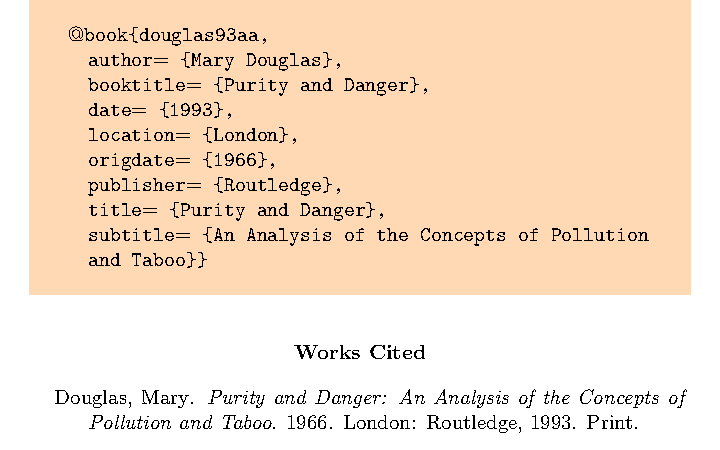
\includegraphics[width=4.8in]{example-book.pdf}
% 	\caption{A standard \sty{.bib} file \mycode{@book} entry and its corresponding output in the list of Works Cited, beneath.}
% 	\label{fig:example-book}
% \end{table}
%
% In addition to many of the standard fields one might expect to find, \biblatexmla is also capable of handling unusual fields, described below. For a fuller consideration of the fields supported by \biblatexmla, see the example files and consult the Biblatex manual.


% \mlafullexample{douglas93aa}{The above entry, found in the \sty{.bib} file, outputs to the below entry in the list of works cited:} %Below are the different \sty{@types} and the fields available to them. Keep in mind that some of the fields in the \sty{@book} and \sty{@article} types (for example, \sty{nameaddon}, \sty{origyear}, and others) are also available in others where it makes sense; I don't repeat them here to save room.

% subsection typical_fields (end)

\subsection{Notable Fields}\label{mla:subsec:unnusualfields}
\biblatex supports the following fields, sometimes concerned more with presentation than bibliographic merit, in all entrytypes. Define these in your \mycode{.bib} files:

\begin{optionslistNOT}
	
	\optionitem{crossref}
	the \sty{key} of a parent source in which a shorter source is found. The \sty{crossref} field is handy to avoid spending time re-inputting similar data, but it is also useful for including \mla{}-style cross-references in the list of Works Cited. Keep in mind the problems of the \sty{crossref} field, explained in section 2.4.1 of the \biblatex manual.% In the future, \biblatexmla may provide further support for the \biblatex \sty{xref} field, making \sty{crossref} secondary in importance.
	
	\optionitem{shorttitle}
	the shortened title to be printed in citations to disambiguate among multiple titles by one author. \Biblatexmla will only print this field in citations when necessary; when this field is not defined, \biblatexmla will use the whole of the \sty{title} field.
	
	\optionitem{shorthand}
	when defined, a unique label to be printed in citations instead of the author and shorttitle. By default, \biblatexmla will only use the \sty{shorthand} label after a first citation with author (and title, if necessary). See the \mycode{firstlonghand} option on page~\pageref{mla:internal:firstlonghand} to disable this feature.
	
	\optionitem{options}
	separate the following options with a comma:
	\begin{description}
		\item[useauthor=false] allows the label of the entry to default to something other than the author, when the author field is defined. If the editor is defined, the label will default to that. The \mycode{useauthor} option defaults to true.
		\item[useeditor=false] allows the label of the entry default to something other than the editor in the case of the author field being undefined or the \mycode{useauthor} option set to false. The \mycode{useeditor} option defaults to true.
		\item[usetranslator=true] allows the label of the entry to inherit the name of the translator when the author and editor fields are undefined or the \mycode{useauthor} and \mycode{useeditor} options are set to false. The \mycode{usetranslator} option defaults to false.
		\item[totalnames=true] allows the label to include all the names in its list, rather than maxing out at three. The \mycode{totalnames} option defaults to false.
		\item[uniquetranslator=true] indicates that a translator of a particular \sty{@incollection} entry is unique to that work, rather than the collection at large. The \mycode{uniquetranslator} option defaults to false.
		\item[noremoteinfo=false] indicates that the ``remote'' information of an entry is to be printed, including the fields \sty{isbn}, \sty{issn}, \sty{isrn}, \sty{doi}, and \sty{eprint}. These fields are usually omitted. See also the global option also called \mycode{noremoteinfo}, on page~\pageref{mla:internal:noremoteinfo}, above, for defining this option on a per-document basis. The \mycode{noremoteinfo} option defaults to true.
	\end{description}	
\end{optionslistNOT}


\subsection{Standalone Sources}
The following entrytypes are for long sources not part of any other publication except, potentially, multivolume sets or publishers' series.

\subsubsection*{@book}
A book, usually with one author. \mla{}-style book entries are straightforward, and the \biblatexmla files style all the potential fields for a typical book

\begin{optionslistNOT}
	\optionitem{author}
	the author of the book

	\optionitem{title}
	book title; when using \sty{crossref}, also define \sty{booktitle} and be sure to define \sty{title} of the child entry

	\optionitem{subtitle}
	book subtitle; when using \sty{crossref}, also define \sty{booksubtitle} and be sure to define \sty{subtitle} of the child

	\optionitem{location}
	entryplace of publication

	\optionitem{publisher}
	publishing house

	\optionitem{date}
	date of publication; defined as \sty{YYYY} for a year, \sty{YYYY-MM} for a month, \sty{YYYY-MM-DD} for a day, or \sty{YYYY-MM-DD/YYYY-MM-DD} for a range
\end{optionslistNOT}

Other fields might come in handy for further granularity:

\begin{optionslistNOT}
	\optionitem{origdate}
	original publication date, for reprints; defined as \sty{YYYY} for a year, \sty{YYYY-MM} for a month, \sty{YYYY-MM-DD} for a day, or \sty{YYYY-MM-DD/YYYY-MM-DD} for a range

	\optionitem{edition}
	edition number

	\optionitem{volume}
	volume number of book

	\optionitem{volumes}
	total number of volumes

	\optionitem{maintitle}
	title of multi-volume collection of which this book is one volume

	\optionitem{mainsubtitle}
	subtitle of the above \sty{maintitle}

	\optionitem{series}
	name of a publication series

	\optionitem{number}
	number of the above \sty{series} represented by this book

\end{optionslistNOT}

Additionally, the style files support more name types for situations needing them:

\begin{optionslistNOT}
	\optionitem{editor}
	editor of a book

	\optionitem{editortype}
	to indicate if the named \sty{editor} is actually an \sty{editor} (``ed.''), a \sty{compiler} (``comp.'') or a \sty{compilerandeditor} (``comp. and ed.''). Default value is \sty{editor}.

	\optionitem{translator}
	translator of a work

	\optionitem{introduction}
	author of a book's introduction

	\optionitem{foreword}
	author of a book's foreword

	\optionitem{afterword}
	author of a book's afterword

	\optionitem{redactor}
	name of redactor

	\optionitem{commentator}
	name of commentator

	\optionitem{annotator}
	name of annotator

\end{optionslistNOT}

Finally, the style files also define the following note fields for further clarification:

\begin{optionslistNOT}
	\optionitem{nameaddon}
	pseudonym, misattribution, or other note (printed in brackets after \sty{author})

	\optionitem{booktitleaddon}
	note after the \sty{booktitle}

	\optionitem{maintitleaddon}
	note after the \sty{maintitle}

	\optionitem{note}
	miscellaneous data printed before \sty{publisher}

	\optionitem{addendum}
	miscellaneous data printed at the end of the entry

\end{optionslistNOT}

Fields not yet supported in biblatex-mla (but which should be supported in future versions) include the following:

\begin{optionslistNOT}
	\optionitem{howpublished}
	to be used in support of the MLA-style revisions in the third edition of the \emph{MLA Style Manual} and the 7th edition of the \emph{MLA Handbook}; will default to ``Print''  when undefined

	\optionitem{origlocation}
	original place of publication (for reprints)

	\optionitem{origpublisher}
	original publisher (for reprints)

	\optionitem{origtitle}
	original title (for reprints)

	\optionitem{origlanguage}
	the original language of a translated, reprinted work. Biblatex-mla will not print information in this field, but if the field has information in it, it will use the phrase ``Trans. of''  before the original title, instead of ``Rept. of''.

\end{optionslistNOT}

\subsubsection*{@booklet}
Small pamphlet, often without an author listed. In \biblatexmla, \mycode{@booklet} is an alias for \mycode{@book} (see above), and is styled similarly.

\subsubsection*{@collection}
A book that is a collection of self-contained essays, stories, or poems, usually with multiple unique authors and collectively edited by a single editorial body. In \biblatexmla, \mycode{@collection} is an an alias for \mycode{@book} (see above), and is styled similarly. To accurately support \mycode{@incollection} entries using \mycode{crossref}, be sure to define the following fields instead of \mycode{title} and \mycode{subtitle} in the parent \mycode{@collection} entry:

\begin{optionslistNOT}
	\optionitem{booktitle}
	the title of a book or collection

	\optionitem{booksubtitle}
	the subtitle of a book or collection

\end{optionslistNOT}

Additionally, remember to define the \mycode{editor} field if needed.

\subsubsection*{@periodical}
An entire issue of a journal, usually cited by editor. \biblatexmla accepts the following fields:

\begin{optionslistNOT}
	\optionitem{editor}
	the editor or editors of an issue

	\optionitem{issuetitle}
	title of a special issue

	\optionitem{issuesubtitle}
	subtitle of a special issue

	\optionitem{title}
	title of the journal

	\optionitem{subtitle}
	subtitle of the journal

	\optionitem{volume}
	volume number

	\optionitem{number}
	issue number

	\optionitem{issue}
	season, when used in place of month (as in the ``spring'' issue of a journal)

	\optionitem{date}
	date of publication, defined as \sty{YYYY} for a year, \sty{YYYY-MM} for a month, \sty{YYYY-MM-DD} for a day, or \sty{YYYY-MM-DD/YYYY-MM-DD} for a range.
	
	\optionitem{pages}
	complete pagination of the issue

\end{optionslistNOT}

\subsubsection*{@proceedings}
The published proceedings of a conference. \Biblatexmla styles \sty{@proceedings} entries like \sty{@book} or \sty{@collection} entries, but it also provides support for the following unique fields:

\begin{optionslistNOT}

	\optionitem{eventtitle}
	
	title of the conference represented by the proceedings (if not included in the \sty{title} of the published proceedings)
	
	\optionitem{organization}
	
	body sponsoring the conference
	
	\optionitem{urldate}
	
	original date of the conference; defined as \sty{YYYY} for a year, \sty{YYYY-MM} for a month, \sty{YYYY-MM-DD} for a day, or \sty{YYYY-MM-DD/YYYY-MM-DD} for a range. Please note that this is an unusual and temporary use of the \sty{urldate} field; in a future version of \biblatexmla, it will change to \sty{eventdate}.
	
	\optionitem{institution}
	
	university or institution hosting the conference
	
	\optionitem{venue}
	
	location of the conference

\end{optionslistNOT}

\subsubsection*{@reference}
A reference book such as a dictionary or encyclopedia, often supporting \sty{@inreference} entries through \sty{crossref} fields. \Biblatexmla styles a \sty{@reference} entry as it would a \sty{@book} entry.

\subsubsection*{@thesis}
The thesis or dissertation resulting from a doctorate or a master's degree, whether published or unpublished. Supports the following fields typical for defining such an entry:

\begin{optionslistNOT}

	\optionitem{author}
	
	the author of the thesis/dissertation
	
	\optionitem{title}
	
	title
	
	\optionitem{subtitle}
	
	subtitle
	
	\optionitem{type}
	
	degree type. \Biblatexmla defines some MLA-style \sty{@thesis} types pre-localized; choose from the following strings to get accurate styling:
	\begin{description}
		\item[phd] for doctorate; prints as ``Diss.'' in English
		\item[dphil] for doctorate; prints as ``Diss.'' in English
		\item[lic] for licentiate; prints as ``Licentiate thesis''
		\item[ma] for master's; prints as ``MA thesis''
		\item[ms] for master's; prints as ``MS thesis''
		\item[msc] for master's; prints as ``MSc thesis''
		\item[mphil] for master's; prints as ``MPhil thesis''
		\item[mlitt] for master's; prints as ``MLitt thesis''
	\end{description}
	
	For all other types not matching the above codes, biblatex- mla will print the type field exactly as entered, respecting all existing capitalization
	
	\optionitem{institution}
	
	name of degree-granting university
	
	\optionitem{date}
	
	date degree awarded, defined as \sty{YYYY} for a year, \sty{YYYY-MM} for a month, \sty{YYYY-MM-DD}

\end{optionslistNOT}

The entry for a @thesis that has been published needs a few additional fields:

\begin{optionslistNOT}
	
	\optionitem{entrysubtype}
	
	\biblatexmla recognizes only two keys in the \sty{entrysubtype} field for the \sty{@thesis}:
	
	\begin{description}
		\item[published] for published theses
		\item[unpublished] for unpublished theses
	\end{description}
	
	any key other than \sty{published} or \sty{unpublished} will be treated as if it were \sty{unpublished}
	
	\optionitem{location}
	
	place of publication
	
	\optionitem{publisher}
	
	publisher
	
	\optionitem{origdate}
	
	date degree was awarded, defined as \sty{YYYY} for a year, \sty{YYYY-MM} for a month, \sty{YYYY-MM-DD}; please note this difference from an unpublished thesis
	
	\optionitem{date}
	
	date of publication, defined as \sty{YYYY} for a year; please note this difference from an unpublished thesis
	
	\optionitem{series}
	
	name of a publication series
	
	\optionitem{number}
	
	number of the above \sty{series} represented by this book
	
\end{optionslistNOT}


%%%%%%
\subsection{Sources within other works}
The following entrytypes are for shorter works (essays, poems, and other things) that are part of another publication. Many have corresponding standalone sources representing the larger work of which they are a part (i.e., \sty{@incollection} and \sty{@collection}). Entries of shorter works can inherit fields of parent entries by using the \sty{crossref} field.

\subsubsection*{@article}
Articles appearing in periodicals in many media, including academic journals, newspapers, and online sources. \Biblatexmla supports the following fields typical of an article in an academic journal:

\begin{optionslistNOT}

	\optionitem{author} author of the article
	
	\optionitem{title} title of the article
	
	\optionitem{subtitle} subtitle of the article
	
	\optionitem{journaltitle} title of journal
	
	\optionitem{journalsubtitle} subtitle of journal
	
	\optionitem{volume} journal volume number
	
	\optionitem{number} journal issue number
	
	\optionitem{issue} season, when used in place of month (as in the ``spring'' issue of a journal)
	
	\optionitem{date} date, defined as \sty{YYYY} for a year, \sty{YYYY-MM} for a month, \sty{YYYY-MM-DD} for a day, or \sty{YYYY-MM-DD/YYYY-MM-DD} for a range
	
	\optionitem{pages} page numbers of the article

\end{optionslistNOT}

For online and newspaper articles, the style provides additional support for the following fields:

\begin{optionslistNOT}
	
	\optionitem{entrysubtype} defines an article's medium, allowing finer control over styling. \Biblatexmla responds to the following keys in the \sty{entrysubtype} field:
	
	\begin{description}
		\item[newspaper] used for newspaper articles
		\item[magazine] used for magazine articles
	\end{description}
	
	online articles are styled by the presence or absence of a \sty{url} field
	
	\optionitem{url} the url address of an online article
	
	\optionitem{urldate} date of access of an online article, defined as \sty{YYYY-MM-DD}
	
	\optionitem{date} date a newspaper article is published, defined as \sty{YYYY-MM-DD} for a day
	
	\optionitem{location} for newspapers lacking a place-name in their title, the city of publication
	
	\optionitem{version} the printing edition of a newspaper (ie, early edition, national edition, etc.)
	
	\optionitem{chapter} the section of a newspaper article if it uses numbers instead of letters; if the newspaper uses letters, combine the letter with the page number (ie, page ``B12'') in the \sty{page} field
	
\end{optionslistNOT}

In addition, the style provides support for the following fields, used in edge cases and unusual circumstances:

\begin{optionslistNOT}

	\optionitem{nameaddon} pseudonym, misattribution, or other note (printed in brackets after author)
	
	\optionitem{titleaddon} note after the title
	
	\optionitem{origdate} year of original publication for a reprinted article
	
	\optionitem{issuetitle} title of the special issue in which it appeared
	
	\optionitem{issuesubtitle} subtitle of the special issue
	
	\optionitem{editor} editor of the special issue
	
	\optionitem{translator} translator of the article
	
	\optionitem{redactor} name of redactor
	
	\optionitem{commentator} name of commentator
	
	\optionitem{annotator} name of annotator
	
	\optionitem{introduction} author of introduction to special issue
	
	\optionitem{foreword} author of foreword to special issue
	
	\optionitem{afterword} author of afterword to special issue
	
	\optionitem{series} name of journal series; define the series name or define as \sty{newseries} or \sty{oldseries} to let \biblatexmla style the series name correctly
	
	\optionitem{note} miscellaneous data to print before the page numbers
	
	\optionitem{addendum} further miscellaneous note at the end of an entry

\end{optionslistNOT}


\subsubsection*{@bookinbook}
A particular kind of \sty{@incollection}. (See below.)

\subsubsection*{@incollection}
A self-contained unit in a \sty{@collection}. Supports the following fields typical of an essay, short story, or poem found in an anthology:

\begin{optionslistNOT}

	\optionitem{author} the author of the work
	
	\optionitem{title} title of the work
	
	\optionitem{subtitle} subtitle of the work
	
	\optionitem{entrysubtype} defines a work's medium, allowing finer control over styling. By default, \sty{@incollection} entries are printed inside quotation marks, like essays, poems, stories, and other shorter works. \Biblatexmla responds to \mycode{book} and \mycode{play} in the \sty{entrysubtype} field, each of which will cause the title to be printed italicized rather than inside quotation marks. Alternatively, set the entry to a \sty{@bookinbook} type for the same effect.
	
	\optionitem{origdate} original publication date of the work, defined as \sty{YYYY}, \sty{YYYY-MM}, or \sty{YYYY-MM-DD}
	
	\optionitem{booktitle} title of the anthology
	
	\optionitem{booksubtitle} subtitle of the anthology
	
	\optionitem{editor} anthology's editor
	
	\optionitem{location} anthology's city of publication
	
	\optionitem{publisher} anthology's publisher
	
	\optionitem{date} date anthology is published, defined as \sty{YYYY}
	
	\optionitem{pages} page numbers of the work

\end{optionslistNOT}

Further fields supported include all of those supported by the @book type.

\subsubsection*{@inproceedings}

A work published in the proceedings of a conference. Supports all the fields of the \sty{@incollection} and \sty{@proceedings} types.

\subsubsection*{@inreference}

A particular type of \sty{@incollection}, potentially without an author. In addition to those fields defined by \sty{@incollection}, \sty{@inreference} adds or refines the following:

\begin{optionslistNOT}

	\optionitem{title} name of entry in reference book
	
	\optionitem{titleaddon} particular definition of the word
	
	\optionitem{booktitle} the title of the reference book

\end{optionslistNOT}

Note that \sty{@inreference} entries do not need to cite page numbers, though they should specify the edition used. If the year and edition fields match, \biblatexmla styles the entry accordingly.

\subsubsection*{@letter}

The \sty{@letter} entry type is only partially supported in \biblatexmla in order to begin work to support it further in the future. It is currently built onto the same backend as \sty{@article} entries, so it will accept additional fields used in that entry type.

\begin{optionslistNOT}

	\optionitem{author} main author of the letter
	
	\optionitem{title} indication of sender and addressee
	
	\optionitem{titleaddon} additional information
	
	\optionitem{pages} pages
	
	\optionitem{origdate} original date letter was sent

\end{optionslistNOT}

\subsubsection*{@review}

A particular type of \sty{@article}, potentially without a title. In addition to those fields defined by \sty{@article}, \sty{@review} adds or refines the following:

\begin{optionslistNOT}

	\optionitem{booktitle} the title of the book being reviewed
	
	\optionitem{bookauthor} the author of the book being reviewed
	
	\optionitem{editor} the editor of the book being reviewed

\end{optionslistNOT}

Note that reviews found in special issues of journals (using the \sty{issuetitle} and \sty{issuesubtitle} fields) are not fully supported yet.

\subsubsection*{@suppbook}

A foreword, introduction, preface, or other supplementary (and often untitled) material to a \sty{@book}. Supports the following fields typical of such a piece:

\begin{optionslistNOT}

	\optionitem{author} author of the piece
	
	\optionitem{title} title of the piece
	
	\optionitem{subtitle} subtitle of the piece
	
	\optionitem{entrysubtype} the type of supplemental material, including subtypes like ``introduction,'' ``foreword,'' and ``Editor's note.''
	
	\optionitem{booktitle} title of the book the piece appears in
	
	\optionitem{booksubtitle} subtitle of the book the piece appears in 
	
	\optionitem{location} city of publication of the book the piece appears in
	
	\optionitem{publisher} publisher of the book the piece appears in
	
	\optionitem{date} date of publication of the book the piece appears in, defined as \sty{YYYY}
	
	\optionitem{pages} page numbers of the piece

\end{optionslistNOT}

Further fields supported include all of those supported by the \sty{@book} type.

\subsubsection*{@suppcollection}

A foreword, introduction, preface, or other supplementary (and often untitled) material to a \sty{@collection}. Supports all the same fields as \sty{@suppbook}.


%%%%%%
\subsection{Other media}

\subsubsection*{@artwork}
The \sty{@artwork} entry type is only partially supported in \biblatexmla in order to begin work to support it further in the future. It is currently built onto the same backend as \sty{@article} entries, so it accepts additional fields used in that entry type.

\begin{optionslistNOT}

	\optionitem{author} artist responsible for the work
	
	\optionitem{title} title of the piece
	
	\optionitem{type} description of the medium. (Please note that this field doesn't yet work with the current version of \biblatexmla, though support will be added to support bibliographies made for \biblatexcms.)
	
	\optionitem{note} additional note on the work
	
	\optionitem{date} date of creation, defined as \sty{YYYY} for a year, \sty{YYYY-MM} for a month, \sty{YYYY-MM-DD} for a day, or \sty{YYYY-MM-DD/YYYY-MM-DD} for a range
	
	\optionitem{institution} institution holding the artwork. (Please note that this field doesn't yet work with the current version of \biblatexmla, though support will be added to support bibliographies made for \biblatexcms.)
	
	\optionitem{location} city of the institution. (Please note that this field doesn't yet work with the current version of \biblatexmla, though support will be added to support bibliographies made for \biblatexcms.)

\end{optionslistNOT}

\subsubsection*{@audio}
The \sty{@audio} entry type is only partially supported in \biblatexmla in order to begin work to support it further in the future. It is currently built onto the same backend as \sty{@article} entries, so it accepts additional fields used in that entry type.

\begin{optionslistNOT}

	\optionitem{author} author or composer of a work
	
	\optionitem{title} title of the speech, song, or other short piece. (Please note that this field doesn't yet work with the current version of \biblatexmla, though support will be added.)
	
	\optionitem{booktitle} title of the opera, cycle, or other larger collection
	
	\optionitem{origdate} date work was originally written. (Please note that this field doesn't yet work with the current version of \biblatexmla, though support will be added.)
	
	\optionitem{maintitle} title of a book containing the work
	
	\optionitem{date} date of publication of work being referenced
	
	\optionitem{publisher} publisher of work being referenced. (Please note that this field doesn't yet work with the current version of \biblatexmla, though support will be added.)
	
	\optionitem{location} city of publisher. (Please note that this field doesn't yet work with the current version of \biblatexmla, though support will be added.)

\end{optionslistNOT}

\subsubsection*{@image}
The \sty{@image} entry type is only partially supported in \biblatexmla in order to begin work to support it further in the future. It is currently built onto the same backend as \sty{@article} entries, so it accepts additional fields used in that entry type.

\begin{optionslistNOT}

	\optionitem{author} creator of the image
	
	\optionitem{title} title of the work
	
	\optionitem{type} description of the medium. (Please note that this field doesn't yet work with the current version of \biblatexmla, though support will be added to support bibliographies made for \biblatexcms.)
	
	\optionitem{note} additional description of the work
	
	\optionitem{date} date of creation
	
	\optionitem{institution} institution holding the work. (Please note that this field doesn't yet work with the current version of \biblatexmla, though support will be added.)
	
	\optionitem{location} city of the institution holding the work. (Please note that this field doesn't yet work with the current version of \biblatexmla, though support will be added.)

\end{optionslistNOT}

\subsubsection*{@music}
This entry type is an alias for \sty{@audio}.

\subsubsection*{@online}
This entry type is an alias for \sty{@article}.

\subsubsection*{@unpublished}
An unpublished manuscript or typescript. \Biblatexmla supports the following fields typical to an unpublished entry:

\begin{optionslistNOT}

	\optionitem{author} author of the work
	
	\optionitem{title} title of a short work (i.e., an essay or poem)
	
	\optionitem{subtitle} subtitle of a short work
	
	\optionitem{booktitle} title of a longer work (i.e., a book or play)
	
	\optionitem{booksubtitle} subtitle of a longer work
	
	\optionitem{titleaddon} description of untitled work
	
	\optionitem{note} further information used to classify the collection; typeset before the \sty{type} field
	
	\optionitem{type} form of the material. \Biblatexmla defines some MLA-style \sty{@unpublished} types pre-localized; choose from the following strings to get accurate styling:
	
	\begin{description}
		\item[manuscript] for the manuscript of a work; printed as ``Ms.'' or ``ms.'' in English
		\item[transcript] for the typescript of a work; printed as ``Ts.'' or ``ts.'' in English
	\end{description}
	
	For all other types not matching the above codes, \biblatexmla will print the type \sty{field} exactly as entered, respecting all existing capitalization
	
	\optionitem{number} identifying number (such as a call number, box, or folio reference) in a library or archive
	
	\optionitem{library} library, archive, or other research institution holding the unpublished work
	
	\optionitem{location} location of the \sty{library}
	
	\optionitem{addendum} extra material printed at the end of an entry

\end{optionslistNOT}

\subsubsection*{@video}
A recording of a movie, television program, etc. \Biblatexmla supports the following fields necessary for a video:

\begin{optionslistNOT}

	\optionitem{title}
	
	title of the work
	
	\optionitem{subtitle}
	
	subtitle of the work
	
	\optionitem{bookauthor}
	
	author of the book on which the video is based
	
	\optionitem{publisher}
	
	distributor
	
	\optionitem{origdate}
	
	original date of release
	
	\optionitem{howpublished}
	
	publishing medium (ie, DVD, videocassette, etc.)

\end{optionslistNOT}

Additionally, \biblatexmla supports the \sty{author}, \sty{editor}, \sty{namea}, \sty{nameb}, and \sty{namec} fields, modified with the \sty{authortype}, \sty{editortype}, \sty{nameatype}, \sty{namebtype}, and \sty{namectype} fields, attuned to the following localization keys:

\begin{optionslistNOT}
	
	\optionitem{$<$x$>$type}
	\begin{description}
		\item[director] director of a work
		\item[screenplay] author of the screenplay
		\item[performer] list of crucial performers
		\item[composer] composer of a soundtrack
		\item[producer] producer of a work
	\end{description}
	
Note that \biblatexmla will print the \sty{author} field before the \sty{title} (styled using the appropriate \sty{authortype} key) unless the field is empty or the \mycode{useauthor} option is false---at which point it will cascade to the \sty{editor} field, unless \emph{it} is undefined or the \mycode{useeditor} option is false. No other name fields will be printed before the title. Except for any printed before the title, these fields will be printed after the title in the following order: \sty{author}, \sty{editor}, \sty{namea}, \sty{nameb}, \sty{namec}.
	
\end{optionslistNOT}

\section{Meta}
\subsection{License}

\biblatexmla is copyrighted \textcopyright\ 2007--2016, by James Clawson. Permission is granted to copy, distribute, and modify this software under the terms of the \lppl, version 1.3: \mylink{http://www.ctan.org/tex-archive/macros/latex/base/lppl.txt}.

\subsection[Feedback]{Feedback}
\label{int:feb}

If you have any questions, requests, or other feedback please email me. My email address is at the top of this document. If you end up improving the code to be more accurate to the \mla{} standard, please be kind to the rest of us and share; I'm very happy to incorporate improvements! If anything works differently than you feel it ought to work, please let me know. Apart from time and my willingness to write documentation, I'm limited only by the problems of which I'm unaware.

\end{document}
